\begin{figure}[htbp]
  \centering

  % --- Subfigure A ---
  \begin{subfigure}{1.0\linewidth}
    \centering
    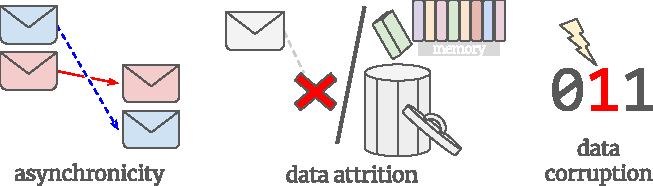
\includegraphics[width=\linewidth,trim={0 0.2cm 0.2cm 0}]{img/best-effort-types.pdf}
    \caption{types of best-effort relaxation}
    \label{moreno:fig:best-effort:types}
  \end{subfigure}

  \vspace{2ex}

  % --- Subfigure B ---
  \begin{subfigure}{1.0\linewidth}
    \centering
    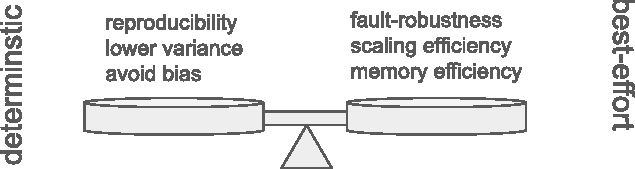
\includegraphics[width=\linewidth,trim={0 -0.2cm 0 0},clip]{img/best-effort-tradeoffs.pdf}
    \caption{practical trade-offs of best-effort relaxations}
    \label{moreno:fig:best-effort:tradeoffs}
  \end{subfigure}

  \vspace{2ex}

  % --- Subfigure C ---
  \begin{subfigure}{1.0\linewidth}
    \centering
    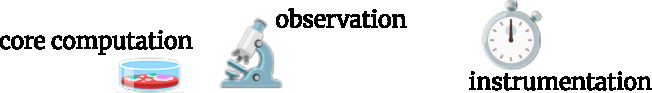
\includegraphics[width=\linewidth,trim={0 -0.2cm 0 0}]{img/best-effort-components.pdf}
    \caption{conceptual components of a best-effort system}
    \label{moreno:fig:best-effort:components}
  \end{subfigure}

  \vspace{2ex}

  % --- Subfigure D ---
  \begin{subfigure}{1.0\linewidth}
    \centering
    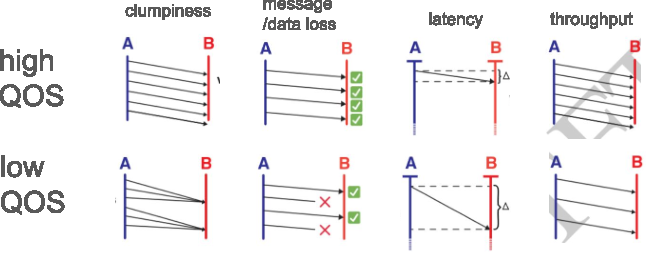
\includegraphics[width=\linewidth,trim={0 -0.2cm 0 0}]{img/best-effort-qos.pdf}
    \caption{dimensions of quality of service (QoS) in best-effort computation}
    \label{moreno:fig:best-effort:qos}
  \end{subfigure}

  \vspace{2ex}

  % --- Main Caption ---
  \caption{
    \textbf{Conceptual framework for best-effort computing.}~%
    Best-effort computing strategies may tolerate asynchronicity, data attrition (e.g., packet loss, dynamic eviction, crashout), or data corruption (panel~\subref{moreno:fig:best-effort:types}).
    While such strategies can improve robustness and efficiency, departing from a reliable deterministic execution model sacrifices computational reproducibility and can degrade computational results by introducing noise and bias (panel~\subref{moreno:fig:best-effort:tradeoffs}).
    In the context of scientific computing, a distinction can be drawn between an \textit{underlying computation} (e.g., a simulation kernel) and \textit{observations} performed to document its behavior (panel~\subref{moreno:fig:best-effort:components});
    to balance efficiency and integrity, best-effort relaxation may be restricted to just data collection (``inferential observability'').
    As a best practice, projects incorporating best-effort strategies should consider \textit{instrumentation} to monitor runtime behavior of relaxations (panel~\subref{moreno:fig:best-effort:components}).
    Panel~\subref{moreno:fig:best-effort:qos} suggests several quality of service metrics that may be collected.
  }
  \label{moreno:fig:best-effort}
\end{figure}
